\Chapter{Kínai karakterek felismerése}

{\large \textbf{Az alapvonások}}

Az írásjegyek felépítésének következő lényeges szabálya az írásjegy vonásainak sorrendje. Az írásjegyek – bármilyen bonyolult legyen is némelyik – tulajdonképpen néhány igen egyszerű vonalból épülnek fel. Ezek az írásjegyek alapelemei, vagy alap-ecsetvonásai. A jobb oldali képen az alapvonások néhány főbb típusa látható. Természetesen az alapvonásoknak több változata is lehetséges (méret, vastagság, irány) attól függően, hogy az írásjegy melyik részén helyezkedik el.

\begin{center}
	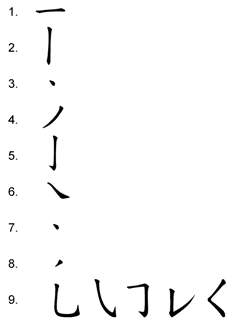
\includegraphics[width=0.4\linewidth]{chinese_strokes}
\end{center}



Minden egyes vonásnak megvan a felépítési szabálya: az ecsetvonásoknak meghatározott sorrendben kell követniük egymást, mégpedig általános elvként az írásjegyek határait alkotó virtuális négyszög bal felső sarkából lefelé és jobbra haladva. Az írásjegy gerincét, fő szerkezeti elemét adó nagyobb vonást, ha az egész írásjegyet átjárja, legutoljára húzzák.

\newpage
{\large \textbf{A vonássorrend szabályai: }}
\begin{enumerate}
	\item A vízszintes vonások megelőzik a függőleges vonásokat.
	\item A balra lejtő vonások megelőzik a jobbra lejtő vonásokat. 
	\item Az írásjegyek írását felülről kell kezdeni. 
	\item Az írásjegyet balról jobbra haladva építik fel. 
	\item A felülről keretezett írásjegyeknél előbb a keretet kell meghúzni. 
	\item Az alulról keretezett írásjegyeknél a keretet legvégül kell meghúzni. 
	\item A teljes keretet mindig legvégül kell bezárni.
\end{enumerate}

Egy szimmetrikus felépítésű írásjegynél előbb a középső részt kell kialakítani, s csak azután az oldalakat.

\begin{center}
\animategraphics[autoplay]{8}{imgpdf/vonasrend_}{0}{35}
\end{center}

A kínai írásjegyek különböző számú alapvonásokból épülhetnek fel. Ezek közül a legegyszerűbb a csupán egyetlen vízszintes vonalból álló „egy” jelentésű \begin{CJK*}{UTF8}{gbsn}
一
\end{CJK*} ji írásjegy. A kínai írásrendszer más, egy vonásból álló írásjegyet nem tartalmaz. Aránylag ritkák a két vonásból álló írásjegyek is, például: \begin{CJK*}{UTF8}{gbsn}
二
\end{CJK*} er„kettő”,
\begin{CJK*}{UTF8}{gbsn}
十
\end{CJK*} si „tíz”,
\begin{CJK*}{UTF8}{gbsn}
人
\end{CJK*} zsen „ember” stb. A hagyományos írásjegyek zöme 15–30 vonásból épül fel (átlagosan 9 vonásból). Esetenként azonban ennél jóval több vonásból álló írásjegyek is előfordulhatnak, melyek tulajdonképpen már több önálló írásjegy összevonásának is tekinthetők. Ritkák ugyan, de léteznek 50 vagy akár 80 vonásból álló írásjegyek is.

